\documentclass[12pt,a4paper]{article}
\usepackage[utf8]{inputenc}
\usepackage{amsmath}
\usepackage{amsfonts}
\usepackage{amssymb}
\usepackage{physics}
\usepackage{graphicx}

\author{Mikael B. Kiste}
\title{FYS-MENA4111 oblig 2}

%\newcommand{\aVec}{\mathbb{R}}

\begin{document}
	\maketitle
	\begin{enumerate}
		\item The face-centered cubic crystal structure of Silicon
		\begin{enumerate}
			\item Figure \ref{fig:fccvec} shows the face-centered cubic crystal structure of Silicon with the three primitive lattice vectors
			\begin{figure}[h]
				\centering
				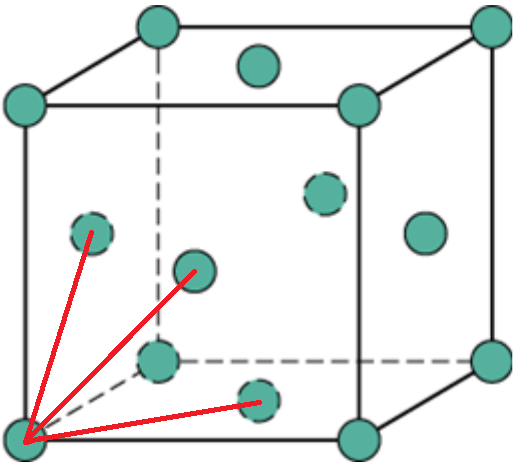
\includegraphics[width=0.7\linewidth]{fccVec}
				\caption{fcc-Si with the three primitive lattice vectors $\vb{a}_1$, $\vb{a}_2$ and $\vb{a}_3$}
				\label{fig:fccvec}
			\end{figure}
			Where
			\begin{align*}
				\vb{a}_1 = \tfrac{a}{2}(\vb{e}_y+\vb{e}_z)\\
				\vb{a}_2 = \tfrac{a}{2}(\vb{e}_x+\vb{e}_z)\\
				\vb{a}_3 = \tfrac{a}{2}(\vb{e}_x+\vb{e}_y)
			\end{align*}
			\item The length of these vectors is
			\begin{align*}
				\abs{\vb{a}_1} = \abs{\vb{a}_2} = \abs{\vb{a}_3} = \abs{\vb{a}_\alpha} = \tfrac{a}{2}\abs{(\vb{e}_y+\vb{e}_z)} = \tfrac{\sqrt{2}}{2}a
			\end{align*}
			\item The reciprocal lattice vectors are defined so that $\vb{a}_i\cdot \vb{a}_j$ is $2\pi$ if $i=j$ and 0 otherwise. This choice means that
			\begin{align*}
				\vb{b_1} = 2\pi \frac{\vb{a}_2\times \vb{a}_3}{\vb{a}_1\cdot (\vb{a}_2\times\vb{a}_3)}\\
				\vb{b_2} = 2\pi \frac{\vb{a}_3\times \vb{a}_1}{\vb{a}_2\cdot (\vb{a}_3\times\vb{a}_1)}\\
				\vb{b}_3 = 2\pi \frac{\vb{a}_1\times \vb{a}_2}{\vb{a}_3\cdot (\vb{a}_1\times\vb{a}_2)}
			\end{align*}
			If we substitute with the expressions for the primitive lattice vectors we can find the primitive reciprocal lattice vectors explicitly.
			\begin{align*}
				\vb{b}_1 = \frac{2\pi}{a}(-1,1,1)\\
				\vb{b}_2 = \frac{2\pi}{a}(1,-1,1)\\
				\vb{b}_3 = \frac{2\pi}{a}(1,1,-1)
			\end{align*}
			\item It is possible to calculate the length of the primitive reciprocal lattice vectors
			\begin{align*}
				\abs{\vb{b}_1} &= \abs{\vb{b}_2} = \abs{\vb{b}_3} = \frac{2\pi\sqrt{3}}{a}
			\end{align*}
		\end{enumerate}
		
		\newpage
		\item Relation between real and reciprocal lattice
		\begin{enumerate}
			\item It can be shown that $\vb{b}_{\alpha}\vb{a}_{\beta} = 2\pi\delta_{\alpha\beta}$. I.e. the dot product between a primitive and real reciprocal lattice vector is $2\pi$ when the indexes are the same and zero otherwise. Let's first assume that $\alpha = \beta$. And let's introduce
			$$c = \vb{a}_1\cdot(\vb{a}_2\cross\vb{a}_3) = \vb{a}_2\cdot(\vb{a}_3\cross\vb{a}_1) = \vb{a}_3\cdot(\vb{a}_1\cross\vb{a}_2)$$
			The general expression becomes
			$$\vb{b}_{\alpha} \vb{a}_{\alpha} = \frac{2\pi}{c}(\vb{a}_{\beta}\times\vb{a}_{\gamma})\vb{a}_{\alpha} = 2\pi$$
			In the other case, when $\alpha \neq \beta$ the dot product can be one of two things
			\begin{align*}
				\frac{2\pi}{c}(\vb{a}_{\beta}\times\vb{a}_{\gamma})\vb{a}_{\beta},
				\qquad \frac{2\pi}{c}(\vb{a}_{\gamma}\times\vb{a}_{\beta})\vb{a}_{\beta}
			\end{align*}
			Which one is the case does not really matter at this point, as the result is the same. Now, we can use the following relation
			\begin{align*}
				\vb{a}_{\alpha}\times\vb{a}_{\beta} = -\vb{a}_{\beta}\times \vb{a}_{\alpha}\\
				(\vb{a}_{\beta}\times\vb{a}_{\gamma})\vb{a}_{\beta} = -(\vb{a}_{\gamma}\times\vb{a}_{\beta})\vb{a}_{\beta}
			\end{align*}
			But the only way for a constant to be equal to the negative of itself is if it is zero. So the product must be zero when $\alpha \neq \beta$
			\item We can use this fact to show that
			\begin{align*}
				\exp(i\vb{G}\cdot\vb{R}) & = \exp(i(n_1m_1\vb{b}_1\vb{a}_1+n_2m_2\vb{b}_2\vb{a}_2+n_3m_3\vb{b}_3\vb{a}_3))\\
				& = \exp(i(n_1m_12\pi+n_2m_22\pi+n_3m_32\pi))\\
				& = \exp(2i\pi l)) = 1
			\end{align*}
			where $n$, $m$ and $l$ are integers
			\item 
		\end{enumerate}
		\newpage
		\item 1D system of particle in infinite square well
		\begin{figure}
			\centering
			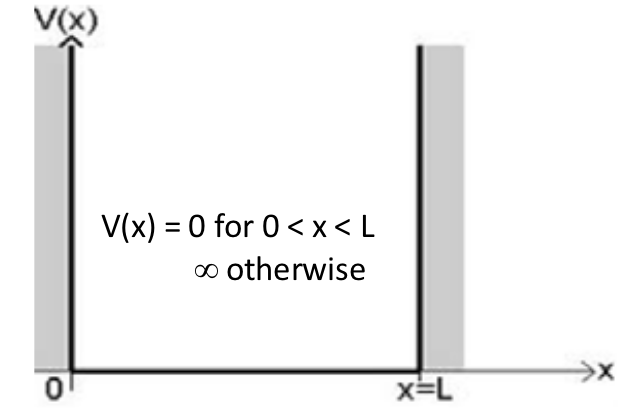
\includegraphics[width=0.7\linewidth]{well}
			\caption{Schematic of an infinite square well potential}
			\label{fig:well}
		\end{figure}
		
		\begin{enumerate}
			\item Finding the solution to the schrödinger equation in such a system is a common exercise
			$$\psi_n(x) = \sqrt{\frac{2}{a}}\sin(\frac{n\pi}{a}x) $$

			\item The three first eigenfunctions can be represented in the well
			\begin{figure}[h]
			\centering
			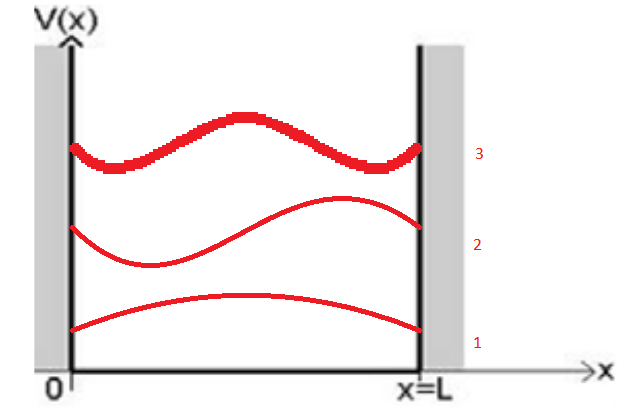
\includegraphics[width=0.7\linewidth]{wellWave}
			\caption{Eigenfunctions $\psi_1$, $\psi_2$ and $\psi_3$}
			\label{fig:wellwave}
			\end{figure}
		
			\item The eigenstates with corresponding energies are given by
			$$ k_n = \frac{n\pi}{a},\qquad E_n = \frac{\hbar^2k_n^2}{2m} $$
			Where n are positive integers.
			\item For plane waves the common relation between wavenumber and wavelength is
			$$k = \frac{2\pi}{\lambda}$$
			\begin{figure}[h]
				\centering
				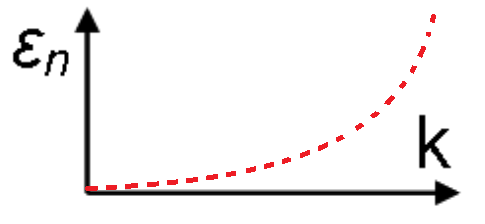
\includegraphics[width=0.7\linewidth]{e(k)Plot}
				\caption{energies as function of the eigenstates $k_n$}
				\label{fig:ekplot}
			\end{figure}
			
		\end{enumerate}
		
	\end{enumerate}

























\end{document}